\documentclass[8pt,t,usepdftitle=false]{beamer}
\usetheme{Juelich}
\usepackage{setspace}
\usepackage[official]{eurosym}
\usepackage{bm}
\usepackage{mathtools}
%\usepackage{enumitem}\setitemize{itemsep=1ex}
\usepackage[%
backend=bibtex,
style=authoryear,
doi=true,
isbn=true,
url=true,
eprint=false,
sorting=nyt]{biblatex}
\addbibresource{refs.bib}

\fzjset{
  title=regular,
  subtitle=regular,
  part=regular,
}

\setbeamerfont{title}{size*={10pt}{10pt},series=\bfseries}
\setbeamerfont{subtitle}{size*={12pt}{12pt},series=\bfseries\color{white}}
\setbeamerfont{frametitle}{size*={14pt}{14pt},series=\bfseries}
\setbeamertemplate{navigation symbols}{}

\setbeamertemplate{itemize/enumerate body begin}{\normalsize}
\setbeamertemplate{itemize/enumerate subbody begin}{\normalsize}
\setbeamertemplate{itemize/enumerate subsubbody begin}{\normalsize}
\setbeamertemplate{itemize/enumerate subsubsubbody begin}{\normalsize}

\mode<presentation>
{
  \usetheme{default}
  %% \setbeamercovered{transparent}
  \usefonttheme{professionalfonts}
  \usefonttheme{structurebold}
  \usecolortheme[rgb={0,0.3,0.6}]{structure}
}

% Delete this, if you do not want the table of contents to pop up at
% the beginning of each subsection:
% \AtBeginSection[]
% {
%   %\begin{frame}<beamer>
%     \begin{frame}[plain]
%     \frametitle{Outline}
%     \tableofcontents[currentsection]
%   \end{frame}
% }

\setlength{\leftmarginii}{3ex}

\setbeamercolor{alerted text}{fg=fzjblue}

\renewcommand{\arraystretch}{1.5}

%%%%%%%%%%%%%%%%%%%%%%%%%%%%%%%%%%%%%%%%%%%%%%%%%%%%%%%%%%%%%%%%%%%%%%%%%%%%%%%%%%%%%%%%%%%%%%%%%
%% macros
\def\figpath{./figures}

\hypersetup{
  pdftitle={Detection of cell assemblies with extracellular multi-electrode recordings},
  pdfauthor={Tom Tetzlaff}
  }

%%%%%%%%%%%%%%%%%%%%%%%%%%%%%%%%%%%%%%%%%%%%%%%%%%%%%%%%%%%%%%%%%%%%%%%%%%%%%%%%%%
\title{%
  {\Large\bf Detection of cell assemblies with extracellular multi-electrode recordings}\\[1ex]
}
\subtitle{%
  {\normalsize\mdseries Tom Tetzlaff}%
  {\hfill\tiny\url{t.tetzlaff{at}fz-juelich.de}}\\
  {\small\mdseries in collaboration with: Alexander Kleinjohann, Sonja Gr\"un, Alessandra Stella, Guenther Palm, David Behrling}\\
  {\footnotesize\mdseries Institute of Neuroscience and Medicine (INM-6), J\"ulich Research Centre and JARA}
  {\hfill\tiny\url{http://www.csn.fz-juelich.de}}
  \\
  {\tiny\mdseries Lab focus, J\"ulich, 11.09.2023}
}
\date{}
\author{}
\institute{}

%%%%%%%%%%%%%%%%%%%%%%%%%%%%%%%%%%%%%%%%%%%%%%%%%%%%%%%%%%%%%%%%%%%%%%%%%%%%%%%%%%%%%%%%%%%%%%%%%
\begin{document}
\maketitle
%%%%%%%%%%%%%%%%%%%%%%%%%%%%%%%%%%%%%%%%%%%%%%%%%%%%%%%%%%%%%%%%%%%%%%%%%%%%%%%%%%%%%%%%%%%%%%%%%
\begin{frame}[plain]
  \begin{center}
    \parbox{0.9\linewidth}{
      \vspace{0.95\textheight}
      \parbox[c]{0.1\linewidth}{%
        \href{https://creativecommons.org/licenses/by-sa/4.0}{%
          
\includegraphics[width=\linewidth]{\figpath/by-sa.png}}}
      \parbox[c]{0.9\linewidth}{\scriptsize%
        ~~{}This presentation is provided under the terms of the Creative Commons Attribution-ShareAlike License 4.0.
      }
    }    
  \end{center}
\end{frame}
%%%%%%%%%%%%%%%%%%%%%%%%%%%%%%%%%%%%%%%%%%%%%%%%%%%%%%%%%%%%%%%%%%%%%%%%%%%%%%%%%%%%%%%%%%%%%%%%%
\def\ttl{Outline}
\pdfbookmark[2]{Outline}{Outline}
\begin{frame}[plain]
  \frametitle{\ttl}
  \tableofcontents
\end{frame}
%%%%%%%%%%%%%%%%%%%%%%%%%%%%%%%%%%%%%%%%%%%%%%%%%%%%%%%%%%%%%%%%%%%%%%%%%%%%%%%%%%%%%%%%%%%%%%%%%
\def\ttl{Background}
\section{\ttl}
%%%%%%%%%%%%%%%%%%%%%%%%%%%%%%%
\def\sttl{Cell assemblies}
\subsection{\sttl}
\begin{frame}[plain]
  \frametitle{\sttl}
  \begin{itemize}
  \item<1-> term ``cell assembly'' coined by \textcite{Hebb49}: ``\ldots network of neurons that is being activated repeatedly during a certain mental process, and in this way, the excitatory synaptic connections among its members are being strengthened\ldots''
    {\tiny\color{gray} \parencite{Abeles11_1505}}
  \end{itemize}
  \vspace*{2ex}
  \onslide<2->{here, more general:}
  \begin{itemize}
  \item<2->  group of neurons that become collectively and \emph{repeatedly} active, and can therefore be reliably \emph{identified} and \emph{labeled} (in the sense ``neuron X is part of assembly Y'')
  \item<2-> a priori, no restrictions on spatial structure and connectivity of cell assemblies, or on temporal structure of assembly activity
  \item<3-> examples:
    \begin{itemize}\itemsep1ex
    \item<3-> neurons that reliably increase their activity level (firing rate) in a task or stimulus specific manner, such as groups of neurons firing in response to their preferred stimulus
      {\tiny\color{gray}\parencite{Hubel59}}
      , or neurons in attractor networks
      {\tiny\color{gray}\parencite{Hopfield82}}
    \item<4-> neurons in a recurrent neuronal network generating spatio-temporal firing patterns in a stimulus or task specific manner, such as neural modes
      {\tiny\color{gray}\parencite{Gallego17_978}}
      , or neurons in networks used for reservoir computing
      {\tiny\color{gray}\parencite{Jaeger01_echo,Maass02_2531,Jaeger04_87}}
    \item<5-> neurons that reliably and recurrently generate spatio-temporal spike patterns with
      high temporal precision, such as neurons in a synfire chain
      {\tiny\color{gray}\parencite{Abeles91}}      
      or in a braid network (polychronous patterns)
      {\tiny\color{gray}\parencite{Bienenstock95,Izhikevich06_245}}      
    \end{itemize}
  \end{itemize}
\end{frame}
%%%%%%%%%%%%%%%%%%%%%%%%%%%%%%%
\def\sttl{Spatiotemporal spike patterns in monkey motor cortex}
\subsection{\sttl}
\begin{frame}[plain]
  \frametitle{\sttl}
  % \framesubtitle{\sttl}
  \begin{itemize}
  \item single-unit spiking activity from reach-to-grasp experiment 
    {\tiny\color{gray}\parencite{Riehle13_48}}
  \item extracellular recordings with $10\times{}10$ Utah array, $400\mu\text{m}$ spacing
  \item identification of spatio-temporal patterns with millisecond precision by SPADE analysis\\
    {\tiny\color{gray}\parencite{Torre13_132,Stella19_104022}}
  \end{itemize}
  \begin{center}
    \parbox{0.7\linewidth}{
      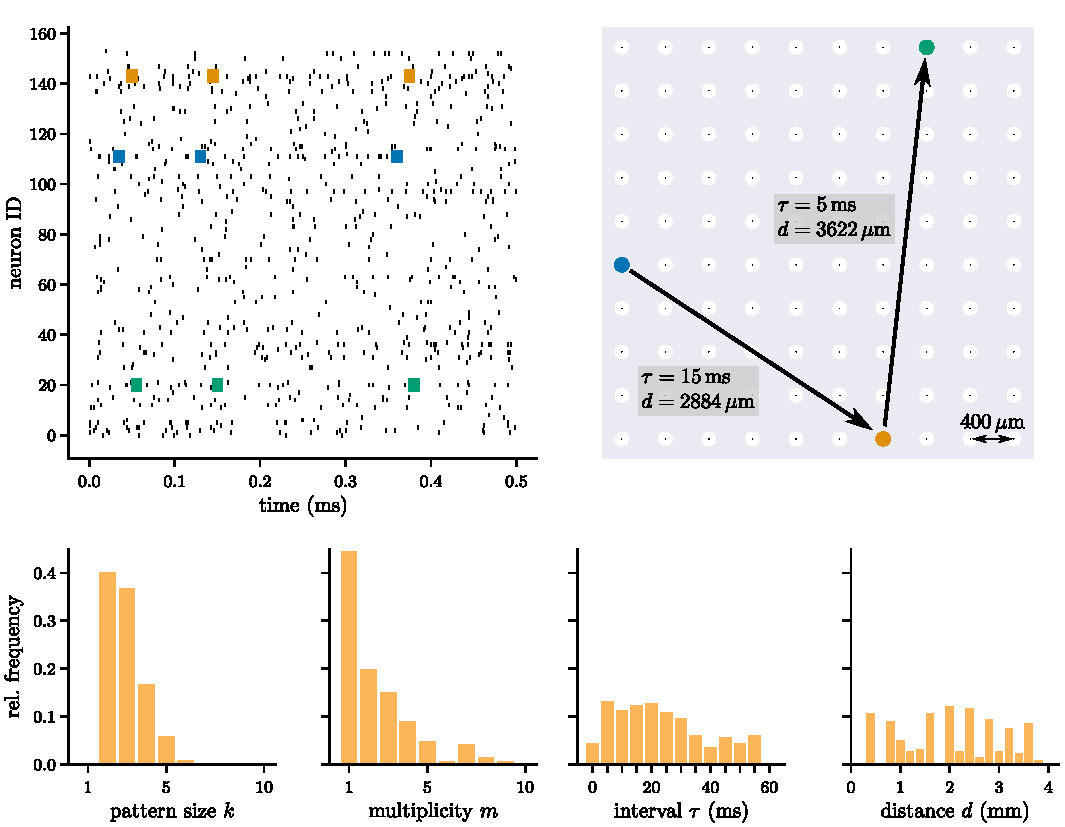
\includegraphics[width=\linewidth]{./figures/graphical_abstract_part_1_mod.pdf}\\
    }    
  \end{center}
  \onslide<2->{
    \vspace*{-4ex}
    \begin{center}
      \emph{
        Neuronal substrate generating such patterns?
        Spatiotemporal structure of these assemblies?
      }      
    \end{center}
  }
\end{frame}
%%%%%%%%%%%%%%%%%%%%%%%%%%%%%%%
\def\sttl{Cell-assembly structure and detectability}
\subsection{\sttl}
\begin{frame}[plain]
  \frametitle{Spatiotemporal cell-assembly structure}
  %\vspace*{-2ex}
  \begin{itemize}
  \item<1-> extracellular multielectrode recordings often suffer from drastic subsampling
  \item<1-> observed spike patterns represent only tip of the iceberg (assemblies)
  \end{itemize}
  \vspace*{1ex}
  \onslide<2->{
    \begin{center}
      \parbox[b]{0.85\linewidth}{\centering
        \emph{What does the rest of the iceberg look like?}\\[1ex]
        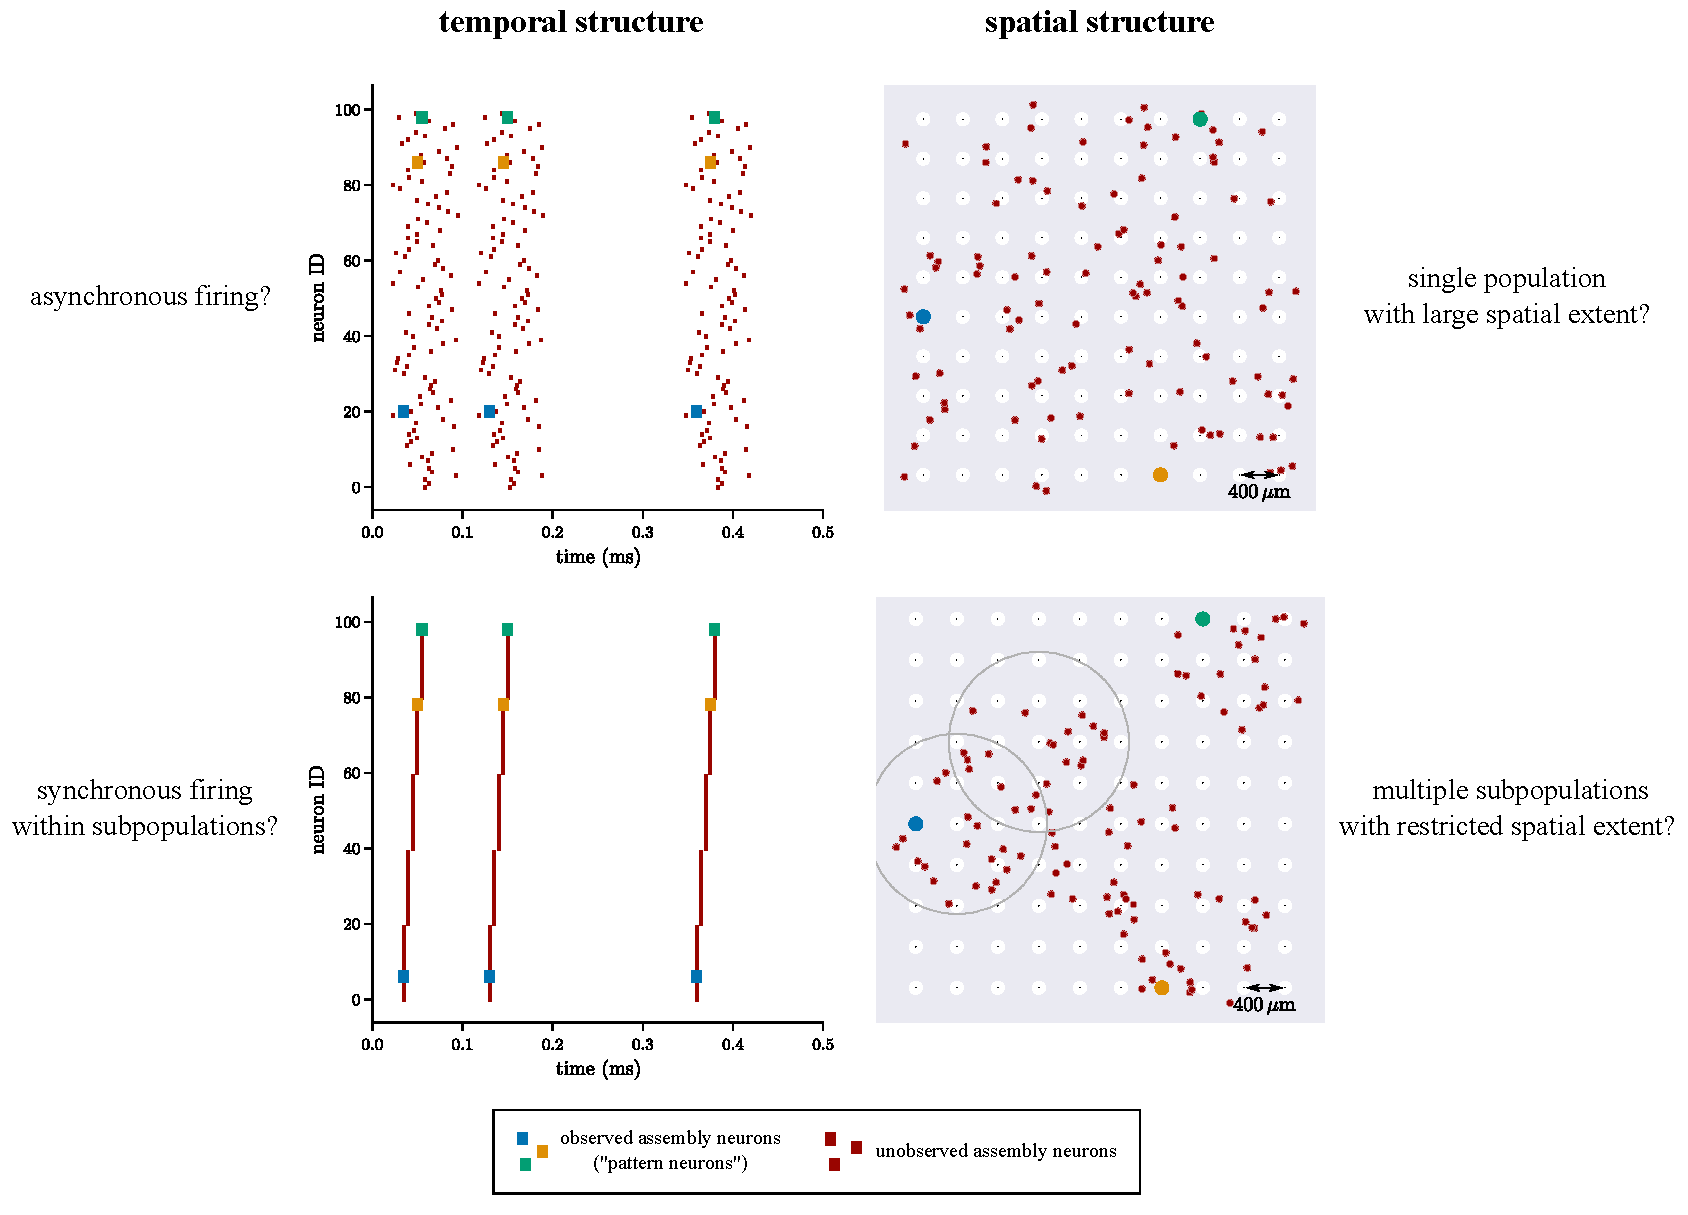
\includegraphics[width=\linewidth]{./figures/graphical_abstract_part_2_mod.pdf}\\
      }%      
    \end{center}
  }%
\end{frame}
\begin{frame}[plain]
  \frametitle{Questions}
  \begin{itemize}
  \item<1-> \emph{Can we infer the cell-assembly structure (e.g., number of neurons, number of assemblies, spatial extent) from knowledge of}
      \begin{itemize}
      \item \emph{the recording constraints, and}
        \item \emph{the statistics of observed patterns?}\\[2ex]
      \end{itemize}
  \item<2-> given a certain recording configuration (e.g., type/number of/distance between electrodes):\\
    \emph{How likely is it to observe cell assemblies with a specific structure?}\\
    (not discussed in this talk)
  \end{itemize}
\end{frame}
%%%%%%%%%%%%%%%%%%%%%%%%%%%%%%%%%%%%%%%%%%%%%%%%%%%%%%%%%%%%%%%%%%%%%%%%%%%%%%%%%%%%%%%%%%%%%%%%%
\def\ttl{Model}
\section{\ttl}
%%%%%%%%%%%%%%%%%%%%%%%%%%%%%%%
\def\sttl{Model of the measurement setup}
\subsection{\sttl}
\begin{frame}[plain]
  \frametitle{\ttl}
  \framesubtitle{\sttl}
  \begin{itemize}
  \item<1-> total number of electrodes $K$ 
  \item<1-> total monitored volume $V$ (volume containing potential cell assemblies), e.g., layer 2/3 below $4\times{}4\,\text{mm}^2$ Utah array
  \item<2-> assume that each electrode can detect neurons within spherical volume $Q=4\pi{}R^3/3$ of radius $R$ surrounding electrode tip (``sensitivity range''; {\tiny\color{gray}\cite{Henze00_390,Pettersen08_784}})
  \item<3->[$\curvearrowright$] expected number $U=\rho{}Q$ of neurons in $Q$ with neuron density $\rho$
  \item<4-> with $\rho\approx{}35000\,\text{neurons}/\text{mm}^3$ {\tiny\color{gray}\parencite{Beul17}}
    and $R\approx{}50\mu\text{m}$: $U\approx{}18$
  \item<5-> empirically {\tiny\color{gray}\parencite{Riehle13_48}}: $U=1.1$
    {\tiny\color{gray}(for an in-depth discussion, see \cite{Shoham06_777})}
  \item<5->[$\curvearrowright$] density of observed neurons $\rho=U/Q\approx{}2100\,\text{neurons}/\text{mm}^3$
  \item<6-> true density of ``eligible'' neurons, i.e., neurons that can potentially participate in an assembly, is unknown and treated as free parameter
  \item<7-> assume that different electrodes have non-overlapping sensitivity ranges (observe disjoint set of neurons)
  \item<7-> probability of detecting some (eligible) neuron:
    \begin{equation*}
      q=\frac{KU}{\rho{}V}
    \end{equation*}
  \item <8-> example: $K=96$, $V=4\times{}4\times{}1.5\,\text{mm}^3$, $U=1.1$
    \begin{equation*}
      q=
      \begin{cases}
        0.0001 & \text{if\quad} \rho=35000\,/\text{mm}^3\\
        0.002 & \text{if\quad} \rho=2100\,/\text{mm}^3
      \end{cases}
    \end{equation*}
    %\item<8->[$\curvearrowright$] \emph{Substantial subsampling!}
  \end{itemize}
\end{frame}
%%%%%%%%%%%%%%%%%%%%%%%%%%%%%%%
\def\sttl{Minimal assembly model}
\subsection{\sttl}
\begin{frame}[plain]
  \frametitle{\ttl}
  \framesubtitle{\sttl}
  \begin{itemize}
  \item<1-> minimal model of spatial arrangement, size and number of assemblies
  \item<1-> no assumptions on network connectivity and dynamics\\[2ex]
  \item<2-> assumptions:
    \begin{itemize}\itemsep1ex
    \item probed volume $V$ contains $A$ cell assemblies
    \item each cell assembly composed of $M$ neurons
    \item assembly neurons are uniformly and independently distributed across $V$
    %\item assembly is ``detected'' if at least two of its neurons are detected
    \end{itemize}
  \end{itemize}
\end{frame}
%%%%%%%%%%%%%%%%%%%%%%%%%%%%%%%%%%%%%%%%%%%%%%%%%%%%%%%%%%%%%%%%%%%%%%%%%%%%%%%%%%%%%%%%%%%%%%%%%
\def\ttl{Pattern statistics}
\subsection{\ttl}
\begin{frame}[plain]
  \frametitle{\ttl}
  % \framesubtitle{\sttl}
  \begin{itemize}
  \item<1-> \emph{pattern size $k$}: probability of detecting $k$ neurons in a given assembly
    \begin{equation*}
      p(k;q,M) = \binom{M}{k}  q^k (1-q)^{M-k}
    \end{equation*}
    with neuron-detection probability $q=KU/\rho{}V$ and assembly size $M$
  \item<2-> \emph{membership multiplicity $m$}: probability of some neuron participating in $m$ different assemblies
    \begin{equation*}
      u(m;b,A)=\binom{A}{m} b^m (1-b)^{A-m}
    \end{equation*}
    with assembly-participation probability $b=M/\rho{}V$ and total number of assemblies $A$ 
  \item<3-> \emph{pattern spike interval $\tau$}: probability of observing time interval $\tau$ between consecutive pattern spikes\\
    \begin{itemize}
    \item not predicted by the minimal model {\footnotesize (ignorant of temporal structure of assembly activity)}
    \end{itemize}
  \item<4-> \emph{pattern neuron distance $d$}: probability of Euclidean distance $d$ between two pattern neurons\\
    \begin{itemize}
    \item[=] frequency of inter-electrode distance $d$
      {\footnotesize (independent + uniform neuron positions within observed volume)}
    \end{itemize}
  \end{itemize}
  \parbox{\linewidth}{ 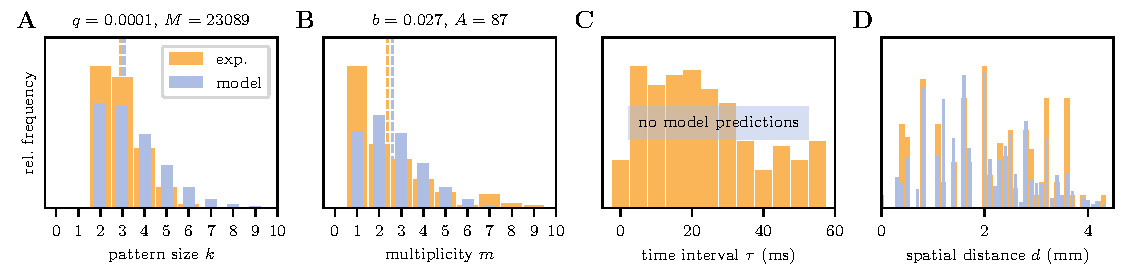
\includegraphics[width=\linewidth]{./figures/minimal_model_stats_rho_35000.pdf}
  }
\end{frame}
%%%%%%%%%%%%%%%%%%%%%%%%%%%%%%%%%%%%%%%%%%%%%%%%%%%%%%%%%%%%%%%%%%%%%%%%%%%%%%%%%%%%%%%%%%%%%%%%% 
\def\ttl{Fitting procedure and results}
\section{\ttl}
\begin{frame}[plain]
  \frametitle{\ttl}
  \begin{itemize}
  %\item fitting pattern-size and multiplicity distributions $p(k;q,M)$ and $u(m;b,A)$ to data from reach-to-grasp experiments
  \item<1-> fix $q=KU/\rho{}V$
    with $K=96$, $U=1.1$, $V=4\times{}4\times{}1.5\,\text{mm}^3$,  $\rho=2100,\ldots,35000\,\text{mm}^{-3}$
    %% $R=50\,\mu\text{m}$
  \item<1-> adjust model parameters $M$, $b=M/\rho{}V$ and $A$ by maximizing sum of normalized model likelihoods
    , i.e., by minimizing cost function
    \begin{equation*}
        E = - S_k^{-1} \sum_{i=1}^{S_k} \text{log}\left[p(k_i;q,M)\right]
      - S_m^{-1}  \sum_{j=1}^{S_m} \text{log}\left[u(m_j;b,A)\right]
    \end{equation*}
    with model distributions $p(\cdot)$ and $u(\cdot)$, empirical pattern sizes and multiplicities $k_i$ and $m_j$, and sample sizes $S_k$ and $S_m$
  \end{itemize}
  \vspace*{2ex}
  \parbox{\linewidth}{
    \onslide<2->{
      \parbox{0.49\linewidth}{%
        $\rho=2100\,\text{mm}^{-3}$:\\[1ex]    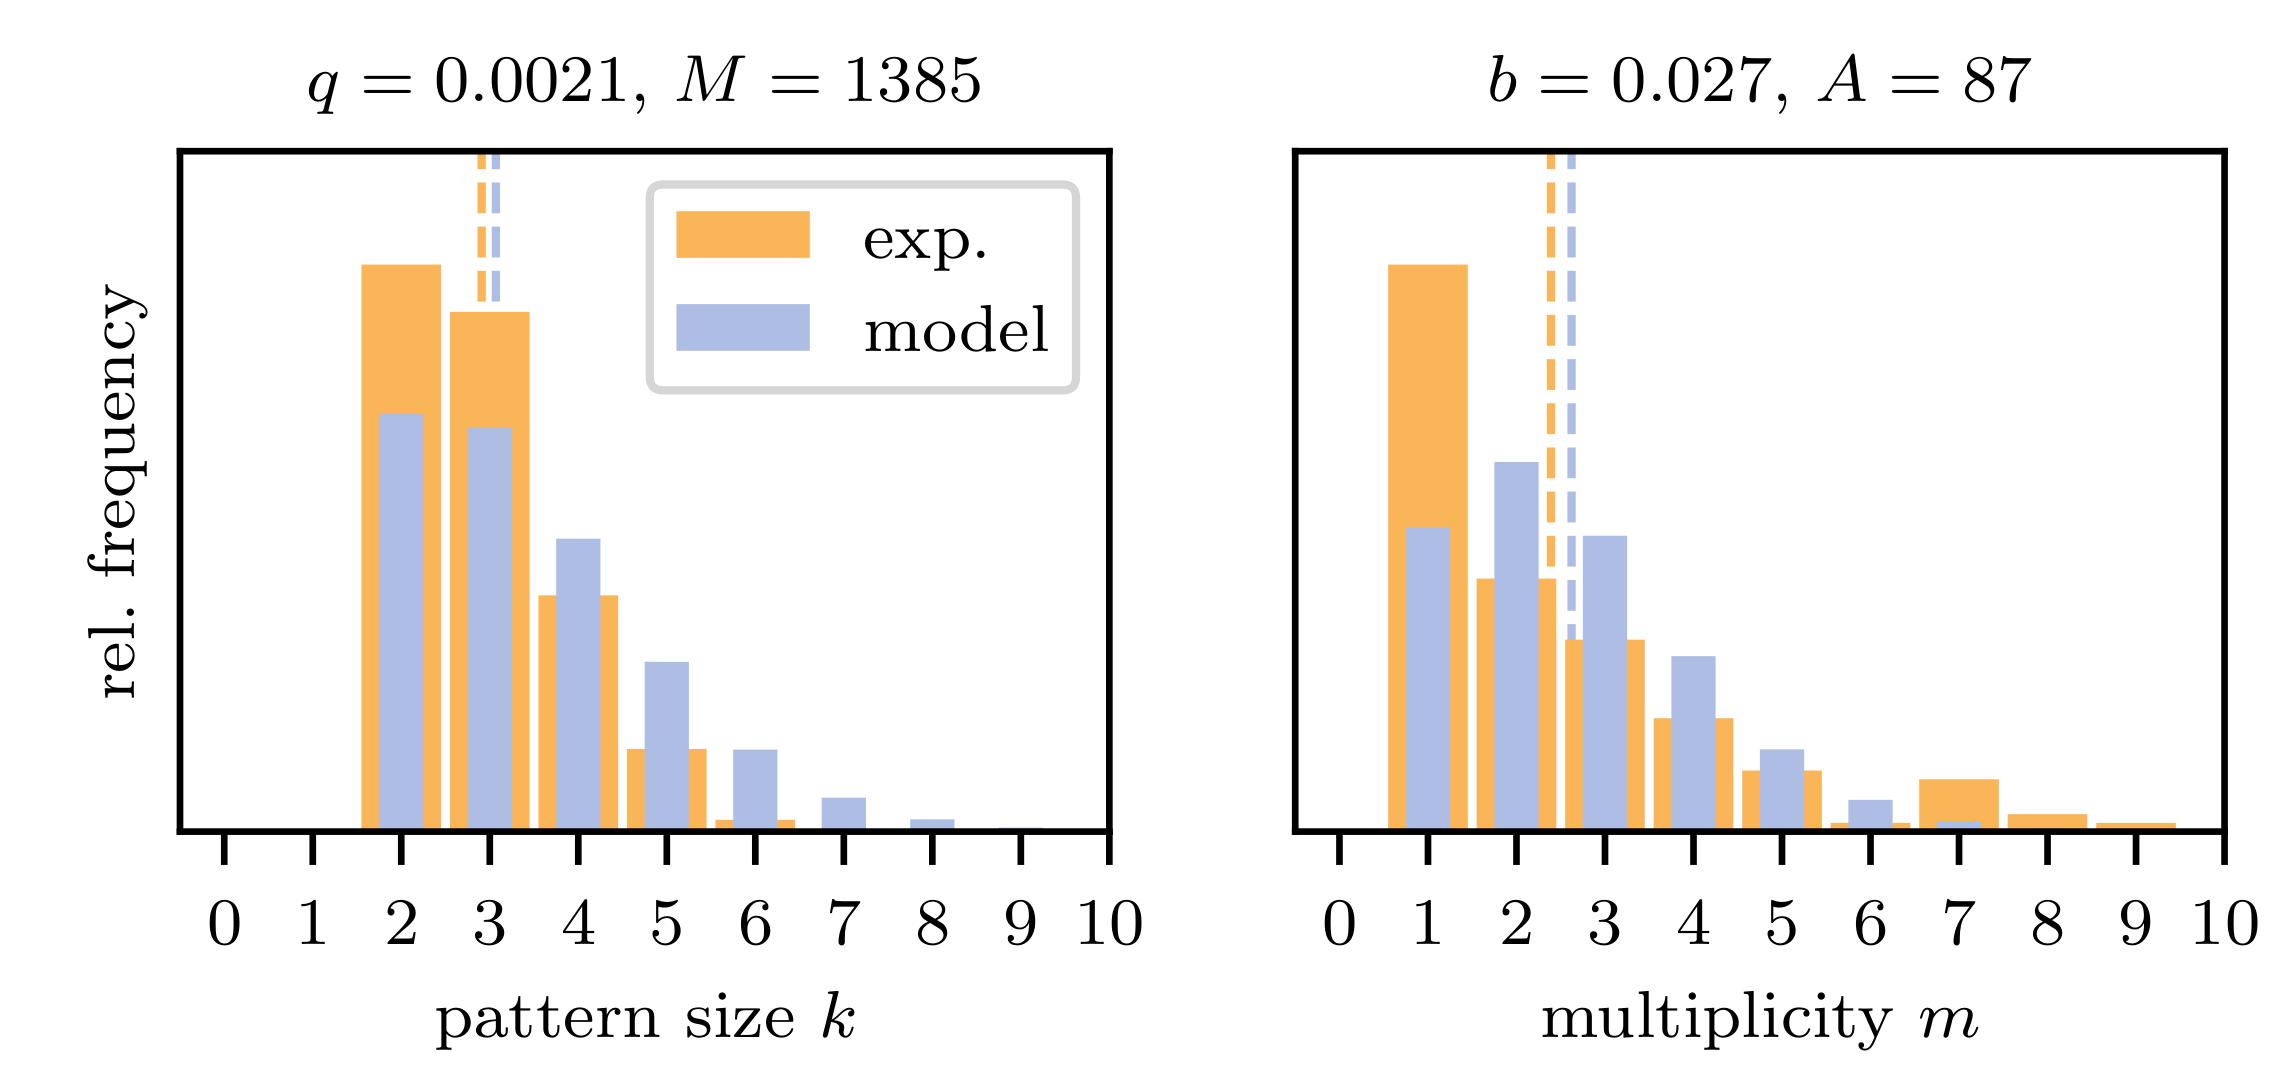
\includegraphics[width=\linewidth]{./figures/minimal_model_stats_rho_2100_AB.png}
      }%
    }%
    \hfill%
    \onslide<3->{    
      \parbox{0.49\linewidth}{%
        $\rho=35000\,\text{mm}^{-3}$:\\[1ex] 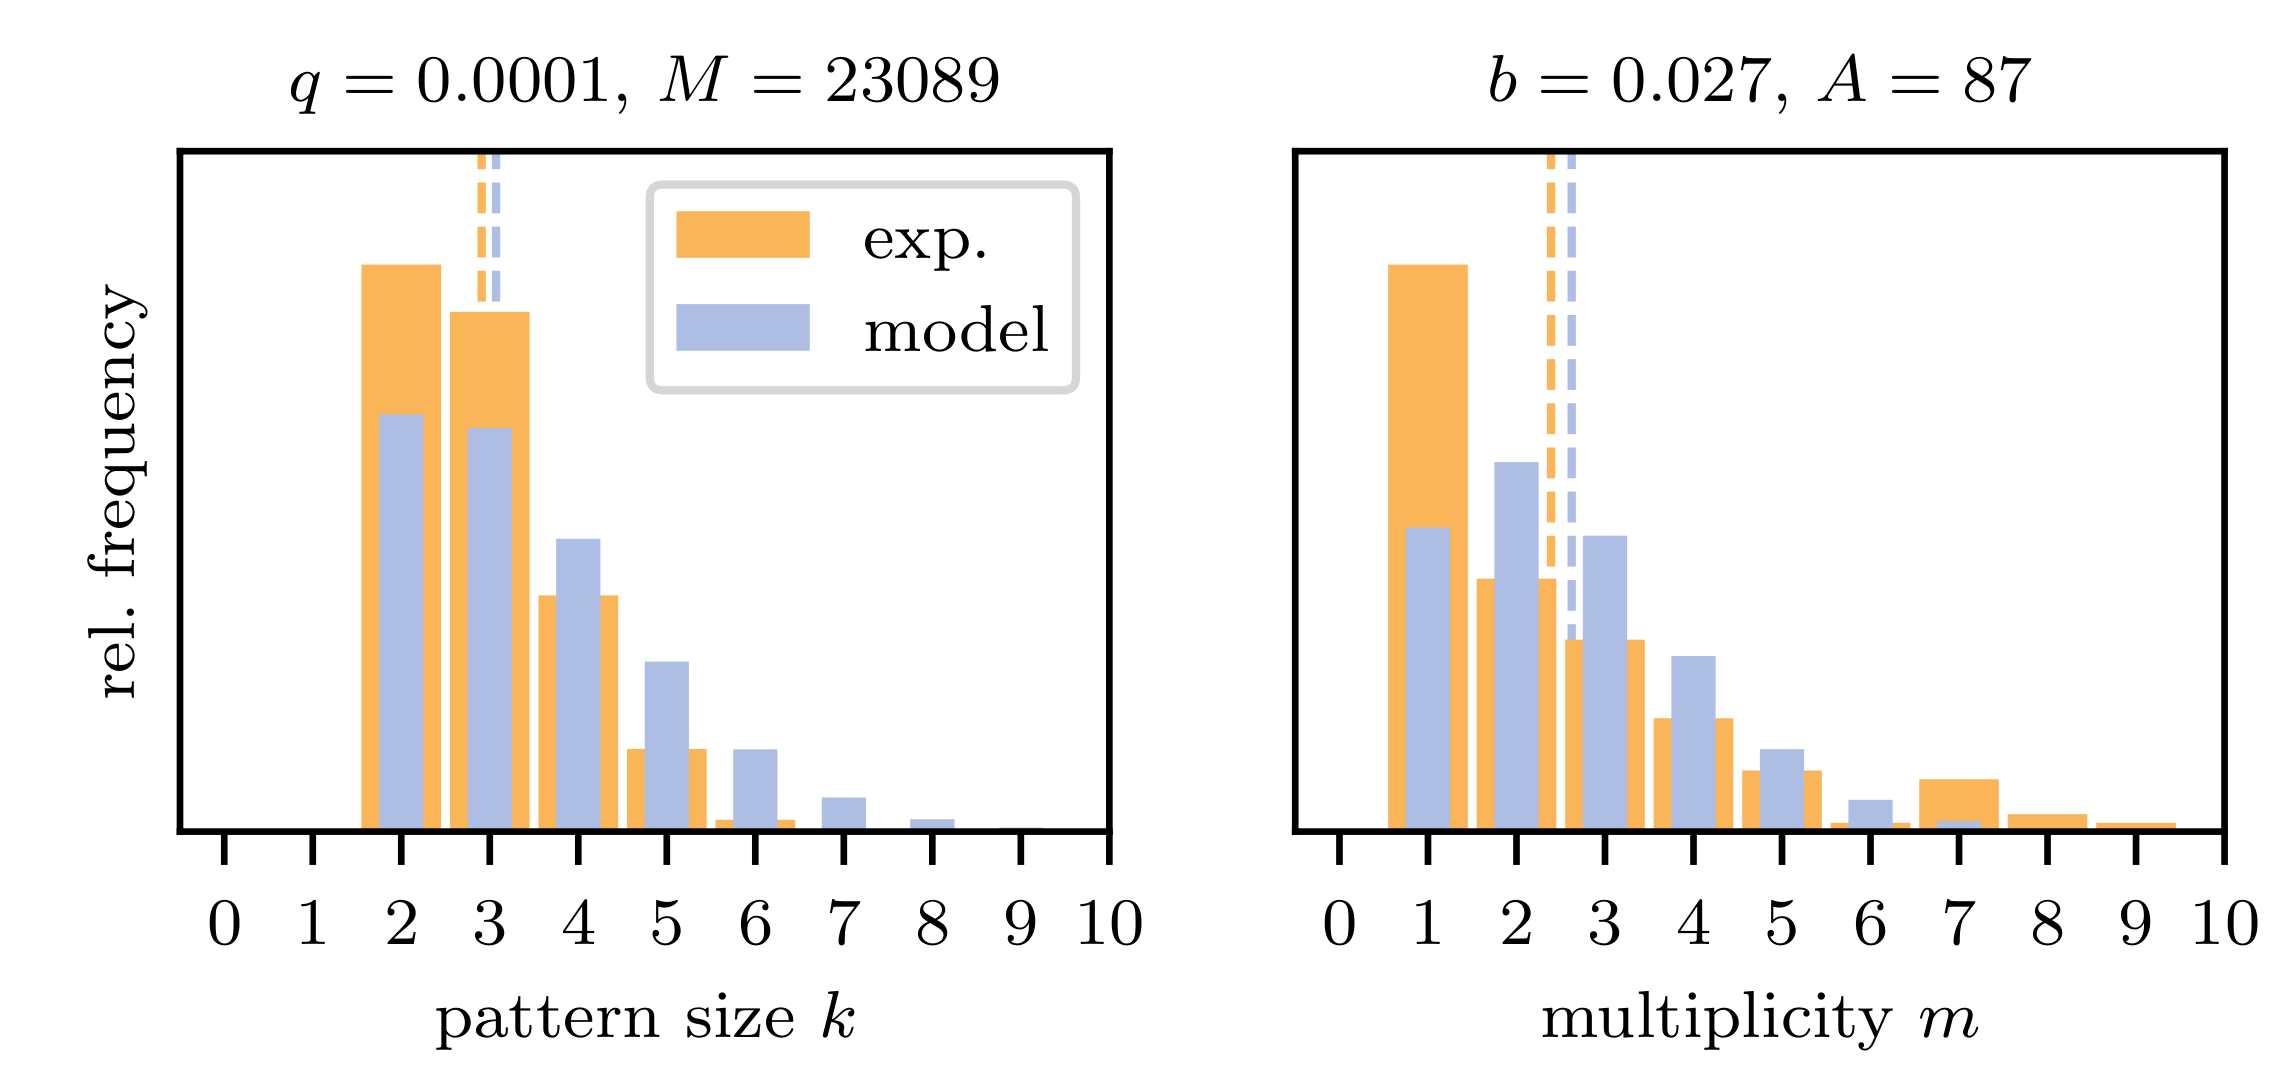
\includegraphics[width=\linewidth]{./figures/minimal_model_stats_rho_35000_AB.png}  
      }
    }
  }
\end{frame}
%%%%%%%%%%%%%%%%%%%%%%%%%%%
\begin{frame}[plain]
  \frametitle{\ttl}
  \begin{itemize}
  \item<1-> best-fit assembly sizes $M$ proportional to $\rho$, with little effect on fit error (same for $V$)
  \item<1-> best-fit assembly participation probability $b=0.027$ and number of assemblies $A=87$ independent of $\rho$
  \end{itemize}
  \vspace*{0.5ex}
  %% 
  {\small\bf best-fit parameters and fit error:}
  \begin{center}
    \parbox{\linewidth}{%
      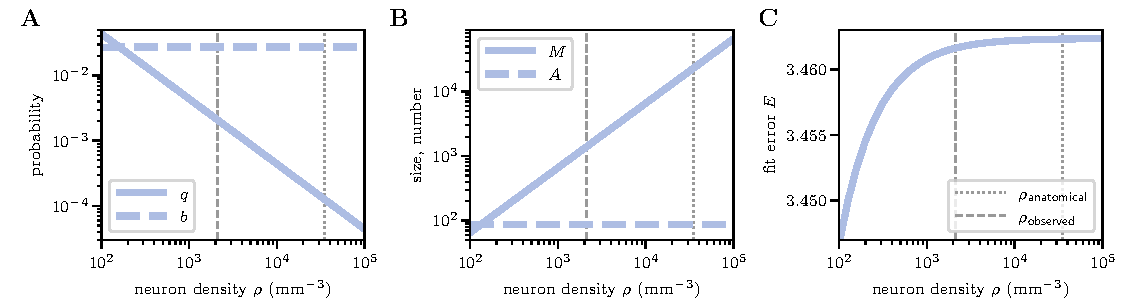
\includegraphics[width=0.9\linewidth]{./figures/minimal_model_fit_range_pars.pdf}
    }
  \end{center}
  %% 
  \only<1>{
    {\small\bf best-fit moments:}
    \begin{center}
      \parbox{0.67\linewidth}{%
        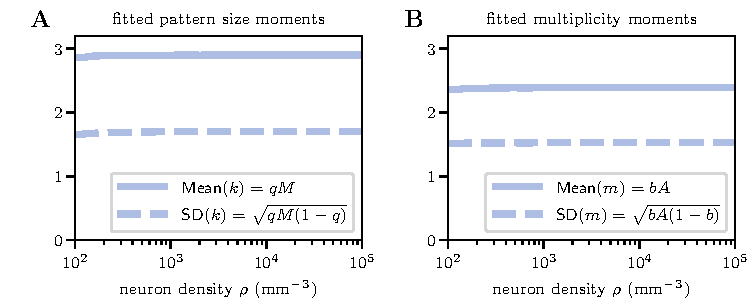
\includegraphics[width=0.9\linewidth]{./figures/minimal_model_fit_range_moments.pdf} 
      }
    \end{center}
  }
  %% 
  \only<2->{
    \vspace*{2ex}
  \fbox{\parbox{\linewidth}{\small%\footnotesize
      explanation: Poisson theorem
      \begin{equation*}
        p(k;q,M) = \binom{M}{k}  q^k (1-q)^{M-k}
        \underset{q\to{}0,Mq=\text{const.}}{\longrightarrow}
        \frac{\lambda^k}{k!}e^{-\lambda{}}
        \quad\text{with}\quad
        \lambda=Mq
      \end{equation*}
      \vspace*{1ex}
      \begin{equation*}
        q=\frac{KU}{\rho{}V}  \quad\curvearrowright\quad
        \lambda=Mq=\frac{MKU}{\rho{}V} \quad\curvearrowright\quad
        M=\frac{\rho{}V\lambda}{KU}  \quad\curvearrowright\quad
        b=\frac{M}{\rho{}V}=\frac{\lambda}{KU}    
      \end{equation*}
    }}}
\end{frame}
%%%%%%%%%%%%%%%%%%%%%%%%%%%%%%%%%%%%%%%%%%%%%%%%%%%%%%%%%%%%%%%%%%%%%%%%%%%%%%%%%%%%%%%%%%%%%%%%% 
% \def\ttl{Assembly detectability}
% \section{\ttl}
% \begin{frame}[plain]
%   \frametitle{\ttl}
%   %\framesubtitle{\sttl}  
% \end{frame}
%%%%%%%%%%%%%%%%%%%%%%%%%%%%%%%%%%%%%%%%%%%%%%%%%%%%%%%%%%%%%%%%%%%%%%%%%%%%%%%%%%%%%%%%%%%%%%%%% 
\def\ttl{Summary}
\section{\ttl}
\begin{frame}[plain]
  \frametitle{\ttl}
  % \framesubtitle{\sttl}
  \begin{itemize}\itemsep1ex
  \item<1-> observations of reach-to-grasp experiment and minimal assembly model hint at presence of
    \begin{itemize}
    \item many ($\sim{}100$) and
    \item large cell assemblies containing $10^3\ldots{}10^4$ neurons
    \end{itemize}
  \item<2-> minimal assembly model and more complex synfire-chain model make similar predictions
  \end{itemize}
  \vspace*{2ex}
  \onslide<2->{
    \parbox{\linewidth}{
      {\bf\small minimal assembly model:}\\    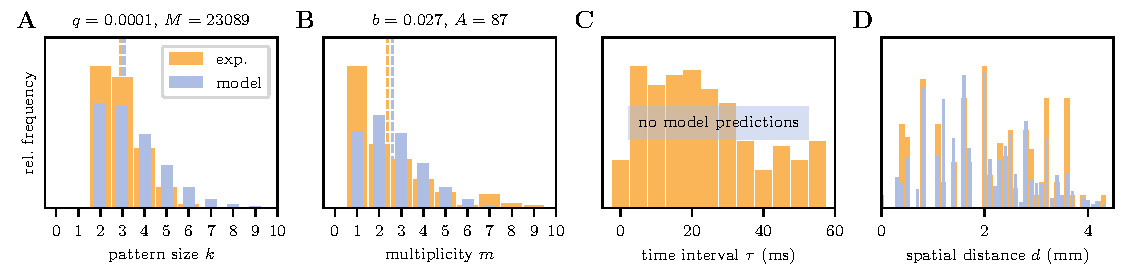
\includegraphics[width=\linewidth]{./figures/minimal_model_stats_rho_35000.pdf}\\
      {\bf\small synfire-chain model:}\\[-4ex]
      \begin{center}
        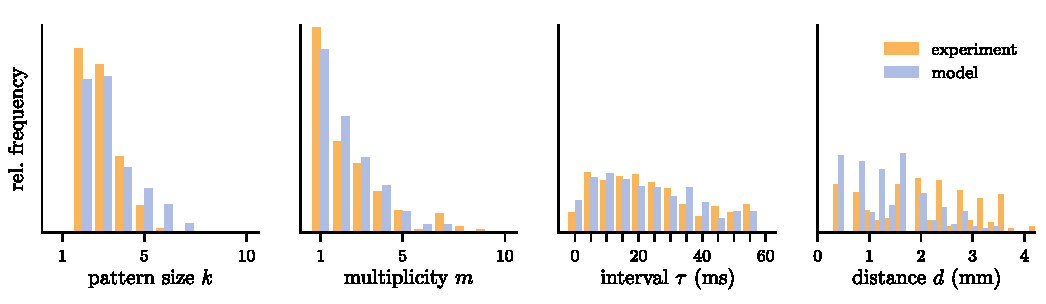
\includegraphics[width=0.95\linewidth]{./figures/sfc_model_stats_mod.pdf}        
      \end{center}
    }}
  \end{frame}
  %%%%%%%%%%%%%%%%%%%%%%%%%%%%%%%%%%%%%%%%%%%%%%%%%%%%%%%%%%%%%%%%%%%%%%%%%%%%%%%%%%%%%%%%%%%%%%%% 
\def\ttl{Outlook}
\begin{frame}[plain]
  \frametitle{\ttl}
  % \framesubtitle{\sttl}
  \begin{itemize}
  \item include minimal model of spike timing (asynchronous firing of assembly neurons) to predict pattern spike interval distributions
  \item quantitative comparison between minimal assembly model and synfire-chain model (use same metrics for fit performance)
  \end{itemize}
\end{frame}
%%%%%%%%%%%%%%%%%%%%%%%%%%%%%%%%%%%%%%%%%%%%%%%%%%%%%%%%%%%%%%%%%%%%%%%%%%%%%%%%%%%%%%%%%%%%%%%%% 
\def\ttl{Ressources}
\section{\ttl}
\begin{frame}[plain]
  \frametitle{\ttl}
  % \framesubtitle{\sttl}
  \begin{itemize}\itemsep2ex
  \item \emph{scientific tools:}\\
    \texttt{python}, \texttt{numpy}, \texttt{scipy}, \texttt{matplotlib}
  \item \emph{workflow tools:}\\
    \texttt{snakemake}
  \item \emph{project locations:}\\
    \url{https://github.com/INM-6/simulate_patterns_from_synfire_chains}\\
    \url{https://github.com/INM-6/synfire_manuscript}    
  \item \emph{data sources:}\\
    pattern characteristics (pattern sizes, multiplicities, pattern spike intervals, pattern neuron distances)\\[1ex]   \url{https://github.com/INM-6/simulate_patterns_from_synfire_chains/blob/master/minimal_assembly_model/py/experimental_results.npy}\\[1ex]
    obtained from reach-to-grasp data \parencite{Riehle13_48}\\[1ex]
    data set: \url{https://doi.gin.g-node.org/10.12751/g-node.f83565}\\
    metadata: \url{https://github.com/INM-6/DataGrasp_Metadata}   
  \item \emph{computing:}\\
    laptop
  \end{itemize}
  \end{frame}
%%%%%%%%%%%%%%%%%%%%%%%%%%%%%%%%%%%%%%%%%%%%%%%%%%%%%%%%%%%%%%%%%%%%%%%%%%%%%%%%%%%%%%%%%%%%%%%%
\begin{frame}[t,plain]
  \begin{center}
    \vspace*{\fill}
    \LARGE\emph{\it Thanks}
    \vspace*{\fill}
  \end{center}
\end{frame}
%%%%%%%%%%%%%%%%%%%%%%%%%%%%%%%%%%%%%%%%%%%%%%%%%%%%%%%%%%%%%%%%%%%%%%%%%%%%%%%%%%%%%%%%%%%%%%%%% 
%% references
\section{References}
\setbeamertemplate{bibliography item}{}  %% remove document icon
\begin{frame}[t,plain,allowframebreaks]  
  \frametitle{References}
  \bibitemsep1ex
  \renewcommand{\bibfont}{\normalfont\small}
  \printbibliography
\end{frame}
%%%%%%%%%%%%%%%%%%%%%%%%%%%%%%%%%%%%%%%%%%%%%%%%%%%%%%%%%%%%%%%%%%%%%%%%%%%%%%%%%%%%%%%%%%%%%%%%%
\section{Appendix}
\begin{frame}[t,plain]
  \begin{center}
    \vspace*{\fill}
    \LARGE \emph{Appendix}
    \vspace*{\fill}
  \end{center}
\end{frame}
%%%%%%%%%%%%%%%%%%%%%%%%%%%%%%%%%%%%%%%%%%%%%%%%%%%%%%%%%%%%%%%%%%%%%%%%%%%%%%%%%%%%%%%%%%%%%%%%%
\def\ttl{Pattern statistics}
\subsection{\ttl}
\begin{frame}[plain]
  \frametitle{\ttl}
  \parbox{\linewidth}{
    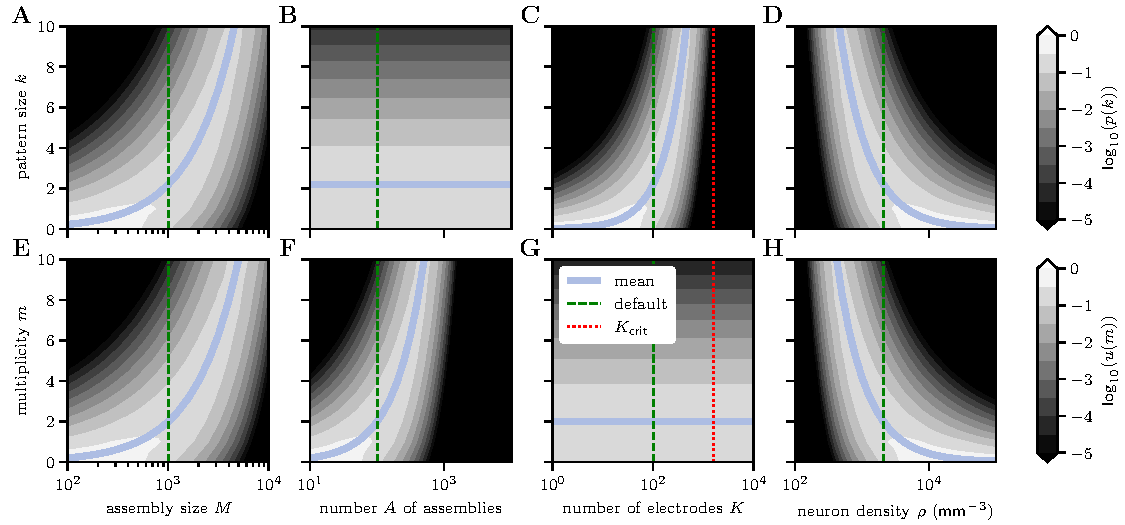
\includegraphics[width=\linewidth]{./figures/minimal_model_stats_3d.pdf}\\
    {\footnotesize
{\bf Pattern statistics predicted by the simple assembly model.} 
%%
Dependence of distributions $p(k)$ and $u(m)$ (contours) of pattern sizes $k$ (A--D) and multiplicities $m$ (E--H)
on the assembly size $M$ (A,E), the number $A$ of assemblies (B,F), the number $K$ of electrodes (C,G), and 
the density $\rho$ of eligible neurons (D,H).
%%
Blue curves represent the mean of the respective distribution.
%%
Dashed green vertical lines depict default parameters (see below).
%%
Dotted red vertical lines in C and G show the maximum number $K_\text{crit}=(L/2R)^2=1600$ of electrodes 
consistent with the assumption of non-overlapping sensivitiy ranges for a Utah array with side length $L=4\,\text{mm}$ 
and electrode sensitivity radius $R=0.05\,\text{mm}$.
%%
Default parameters: $V=24.0\,\text{mm}^3$ , $\rho=2100\,\text{mm}^{-3}$, $K=100$, $U=1.1$, $M=1000$, $A=100$.
%%
    }
  }
\end{frame}
%%%%%%%%%%%%%%%%%%%%%%%%%%%%%%%%%%%%%%%%%%%%%%%%%%%%%%%%%%%%%%%%%%%%%%%%%%%%%%%%%%%%%%%%%%%%%%%%
\def\ttl{Assembly detectability}
\subsection{\ttl}
\begin{frame}[plain]
  \frametitle{\ttl}
  \vspace*{-1ex}
  \begin{itemize}
  \item definition: an assembly is \emph{detected} if at least two of its neurons are detected
  \item single-assembly detection probability:
    \begin{equation*}
      P_1(q,M) = 1 - p(k=0) - p(k=1) = 1 - (1-q)^M - M q (1-q)^{M-1}.
    \end{equation*}
  \item probability of observing at least one assembly within an ensemble of $A$ assemblies:
    \begin{equation*}
      P_A = 1 - (1-P_1)^A.
    \end{equation*}
  \end{itemize}
  \only<1>{
    \parbox{\linewidth}{
      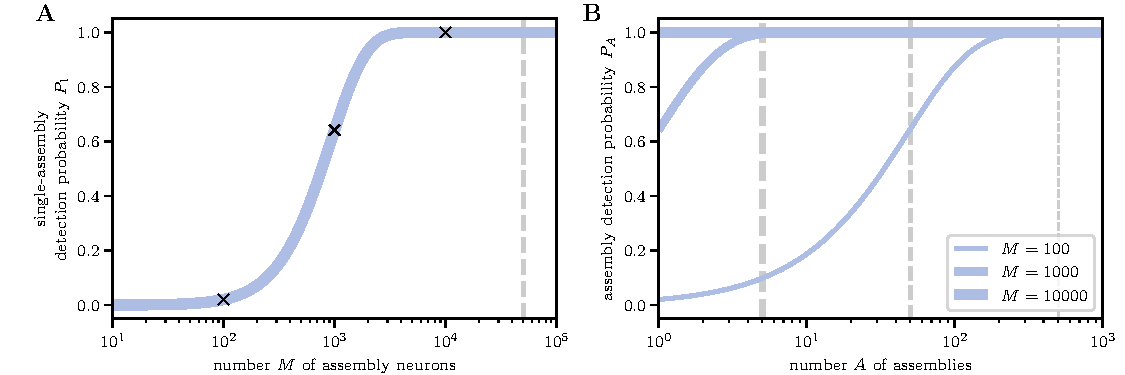
\includegraphics[width=0.9\linewidth]{./figures/minimal_model_assembly_detectability_rho_2100.pdf}\\
      {\footnotesize
{\bf Assembly detectability.} 
%%
{\bf A}: Dependence of the probability $P_1$ of detecting a specific assembly (two or more neurons
in this assembly) on the assembly size $M$.
The dashed vertical gray line marks the point where the number $M = \rho{}V$ of assembly neurons equals the total number of eligible neurons within the observed volume $V$.
The crosses mark the assembly sizes $M$ used in panel B.
%%
{\bf B}: Dependence of the probability $P_A$ of detecting one or more assemblies on the number $A$ of assemblies for different assembly sizes $M$ (see legend).
The dashed vertical gray lines indicate where $MA = \rho{}V$. Latest at this point, assemblies start to overlap.
%%
Default parameters: $V=24.0\,\text{mm}^3$ , $\rho=2100\,\text{mm}^{-3}$, $K=100$, $U=1.1$, $M=1000$, $A=100$.
%%
    }
    }
  }
  \only<2->{
    \parbox{\linewidth}{
      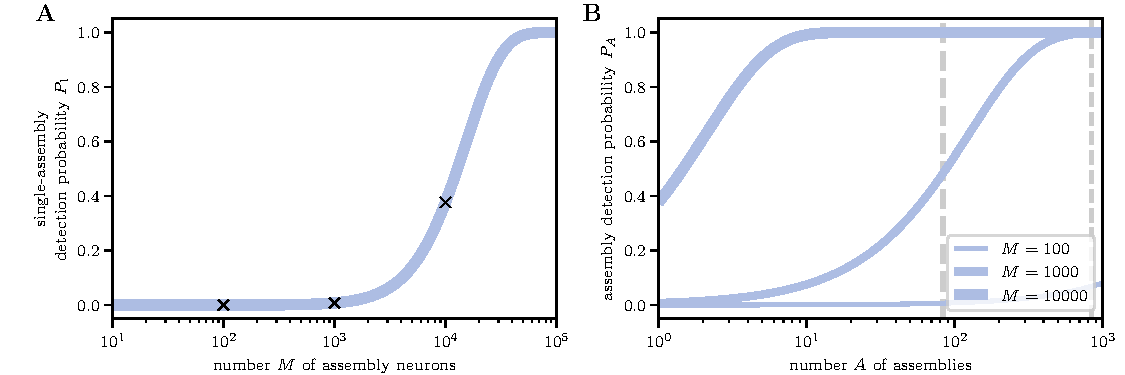
\includegraphics[width=0.9\linewidth]{./figures/minimal_model_assembly_detectability_rho_35000.pdf}\\
      {\footnotesize
{\bf Assembly detectability.} 
%%
{\bf A}: Dependence of the probability $P_1$ of detecting a specific assembly (two or more neurons
in this assembly) on the assembly size $M$.
The dashed vertical gray line marks the point where the number $M = \rho{}V$ of assembly neurons equals the total number of eligible neurons within the observed volume $V$.
The crosses mark the assembly sizes $M$ used in panel B.
%%
{\bf B}: Dependence of the probability $P_A$ of detecting one or more assemblies on the number $A$ of assemblies for different assembly sizes $M$ (see legend).
The dashed vertical gray lines indicate where $MA = \rho{}V$. Latest at this point, assemblies start to overlap.
%%
Default parameters: $V=24.0\,\text{mm}^3$ , $\rho=35000\,\text{mm}^{-3}$, $K=100$, $U=1.1$, $M=1000$, $A=100$.
%%
    }
    }
  }
\end{frame}
%%%%%%%%%%%%%%%%%%%%%%%%%%%%%%%%%%%%%%%%%%%%%%%%%%%%%%%%%%%%%%%%%%%%%%%%%%%%%%%%%%%%%%%%%%%%%%%%%
\end{document}
%%%%%%%%%%%%%%%%%%%%%%%%%%%%%%%%%%%%%%%%%%%%%%%%%%%%%%%%%%%%%%%%%%%%%%%%%%%%%%%%%%%%%%%%%%%%%%%%
%%% Local Variables:
%%% mode: latex
%%% TeX-master: t
%%% End:
